\documentclass[12pt]{report}
\usepackage{parskip}
\usepackage{adjustbox}
\usepackage{amstext}
\graphicspath{ {./images/} }
\usepackage{hyperref}

%\usepackage{amsmath}

\begin{document} 

\begin{titlepage}
\includegraphics[height=2.25cm,keepaspectratio]{lab.png}\hfill \includegraphics[height=2.25cm,width = 3.75cm]{pes.png}

\begin{center}
\vspace*{1cm}

\textbf{\Large{PES Innovation Lab}}

\vspace{0.3cm}
\text{\Large{Project Report}}
\vspace{0.1cm}
       
\text{\Large{Summer Internship 2023}}
       
\vspace{0.8cm}
\text{\huge{BIT* Connect}}
            
\vspace{0.8cm}
\text{\large{Interns}}
       
\vspace{0.2cm}
       
\begin{tabular}{c c}    
    \textbf{Name} & 
    \textbf{SRN} \\[0.5cm]
    \ {Ayush Kale} & {PES2UG21CS107} \\
    \ {Varuni H K} & {PES2UG21CS597} \\
    \ {Vikas Paul Menezes} & {PES2UG21CS606} \\         
\end{tabular}
\vspace{0.5cm}

\text{\large{Mentors}}
\vspace{0.2cm}
       
\begin{tabular}{c c}
    \textbf{Name} & 
    \textbf{SRN} \\[0.5cm]
    \ {SriKrishna B R} & {PES1201700469} \\
    \ {Disha Jain} & {SRN-2} \\
\end{tabular}
       
\vfill
\vspace{0.5cm}
            
PES Innovation Lab\\
PES University\\
100 Feet Ring Road,\\
BSK III Stage,\\
Bangalore - 560085
            
\end{center}
\end{titlepage}


\begin{abstract}
  \font This project aims to combine two motion planning algorithms, \textbf{BIT*} and \textbf{RRT-Connect}, to create a more optimal algorithm called BIT* Connect.\\
  \textbf{RRT-Connect} is a bidirectional planner that finds solutions quickly but may explore unnecessary regions, resulting in suboptimal solutions. \textbf{BIT*(Batch Informed Trees)} is an efficient planner that uses an ellipse-shaped guiding function and guarantees the shortest path.\\
  Our goal is to create an asymptotically optimal algorithm that quickly finds initial and final solutions. By leveraging the efficiency of BIT* and the speed of RRT-Connect, BIT* Connect aims to be a faster and more optimal motion planning algorithm.
\end{abstract}

\tableofcontents
%\listoffigures
%\listoftables

\chapter{Introduction}
Autonomous robotic systems operating in dynamic and unknown environments face a fundamental challenge: navigating between positions. The complexity of this task depends on the vast number of potential robot positions, forming a search space that is often continuous, unbounded, and high dimensional. To address this, most global path-planning algorithms resort to discretization, reducing the search space to a countable subset of states. While this simplifies the problem, it limits algorithm performance to the chosen discrete approximation. In this report, we examine the implications of discretization in path-planning algorithms and explore alternative methods to enhance accuracy and efficiency. By analyzing existing research, we aim to contribute insights for advancing path planning in autonomous robotic systems, enabling them to operate effectively in diverse environments.


RRT-Connect is one such algorithm that is a bidirectional motion planner and finds a solution faster than other planners. However, the algorithm wastes resources exploring regions leading to low-quality solutions and it also doesn’t guarantee the most optimal solution. 


BIT* is another such motion planning algorithm that uses an ellipse-shaped guiding function for exploration toward the goal. It also provides the shortest path possible, thus making it Asymptotically Optimal.


The goal is to improve BIT* and make it faster. This can be done by making it Bidirectional and incorporating the Connect function, while still using the ellipse-shaped guiding function for exploration toward the goal.
\section{Problem Statement}
In this report, we are trying to create a new Path-Planning Algorithm, BIT*Connect that combines BIT* and RRT-Connect to give us a Bidirectional planner and is Asymptotically Optimal.


This report consists of Literature Survey, Software Requirements and ends with the Results and Conclusions that we have arrived at.


\chapter{Literature Survey/Related Work} 
% Length: [1-3 pages]. 
% Are there existing solutions to your problem? If yes, elaborate in a few lines. You can also write about the theory/concepts associated with your project. Cite related work  \cite{wiki:latex}.  You can conclude this section by stating how your work is novel/different from the related work you have just described. For each paper or link that you mention here, please include a short summary of the resource as well as how the resource contributed to your project.
Motion planning is a critical research field in robotics, tackling the complex task of finding feasible paths for robots. Among the various approaches, sampling-based methods have emerged as efficient solutions to address this challenge\cite{lavalle2006planning}. These methods provide a practical way to navigate through intricate environments by sampling configurations and constructing paths based on these samples. Path planning is a purely geometric process that is only concerned with finding a collision free path regardless of the feasibility of the path. Kinodynamic planning, on the other hand, considers the kinematics and dynamics of the robot. Once a path is specified the final procedure is motion control or execution \cite{6722915}.


Probabilistic Roadmaps \cite{508439} constructs a roadmap by randomly sampling configurations and connecting them to form a graph representation of the environment. It then uses graph search algorithms to find a path between the start and goal configurations. This algorithm does not give the optimal solution every time. Considering a configuration space with a large number of obstacles situated very close to each other, if the gap between two obstacles is very narrow, due to our system generates nodes randomly, the probability of generating nodes between those gaps is very small. The system might generate nodes in that region if we increase the number of iterations but increasing the number of iterations does not solve the problem.
When the system fails to generate a path for such configurations of the space, we wouldn’t know whether it is because the path does not exist or the number of iterations is less for that environment.

This problem was overcome by Rapidly Exploring Random Trees (RRT) . RRT* is an improvemnt over RRT as it is asymtotically optimal by introcucing incremental rewiring\cite{6942976} but suffers from high memory consumption due to large expansion of its search space.\cite{noreen2016optimal}Informed RRT* , uses a necessary condition to improve the solution at any iteration by the addition of states from an ellipsoidal subset of the planning domain. \cite{6942976} This helps to focus the search contrary to RRT* which spends a lot of time exploring . The Fast Marching Tree (FMT*) algorithm performs a "lazy" dynamic programming recursion on a predetermined number of probabilistically-drawn samples to grow a tree of paths, which moves steadily outward in cost-to-arrive space \cite{janson2015fast}.

Batch Informed Trees (BIT*), is a planning algorithm that balances the benefits of graph-search and sampling-based techniques. It uses batches of samples to perform an ordered search on a continuous planning domain while maintaining anytime performance. By processing samples in batches, its search can be ordered around the minimum solution proposed by a heuristic, as in A* \cite{7139620}. BIT* is a combination of FMT* and Inforemd RRT* and performs better than all of its predecessors . 

RRT Connect is a bidirectional Motion planner which solves single-query path planning problems in high-dimensional configuration spaces by incrementally building two rapidly-exploring random trees (RRTs) rooted at the start and the goal configurations. The trees each explore space around them and also advance towards each other through, the use of a simple greedy heuristic\cite{844730}.

In this project we propose to combine BIT* and RRT-Connect and give rise to a new algorithm called BIT* Connect which uses the greedy heuristic of RRT - Connect and grow two BIT* trees from both the start and goal states alternatively . RRT Connect gives us the fastest initial solutions and BIT* gives us asymptotic optimality , finding the intial and final (shortest) solution quicker than other planners.


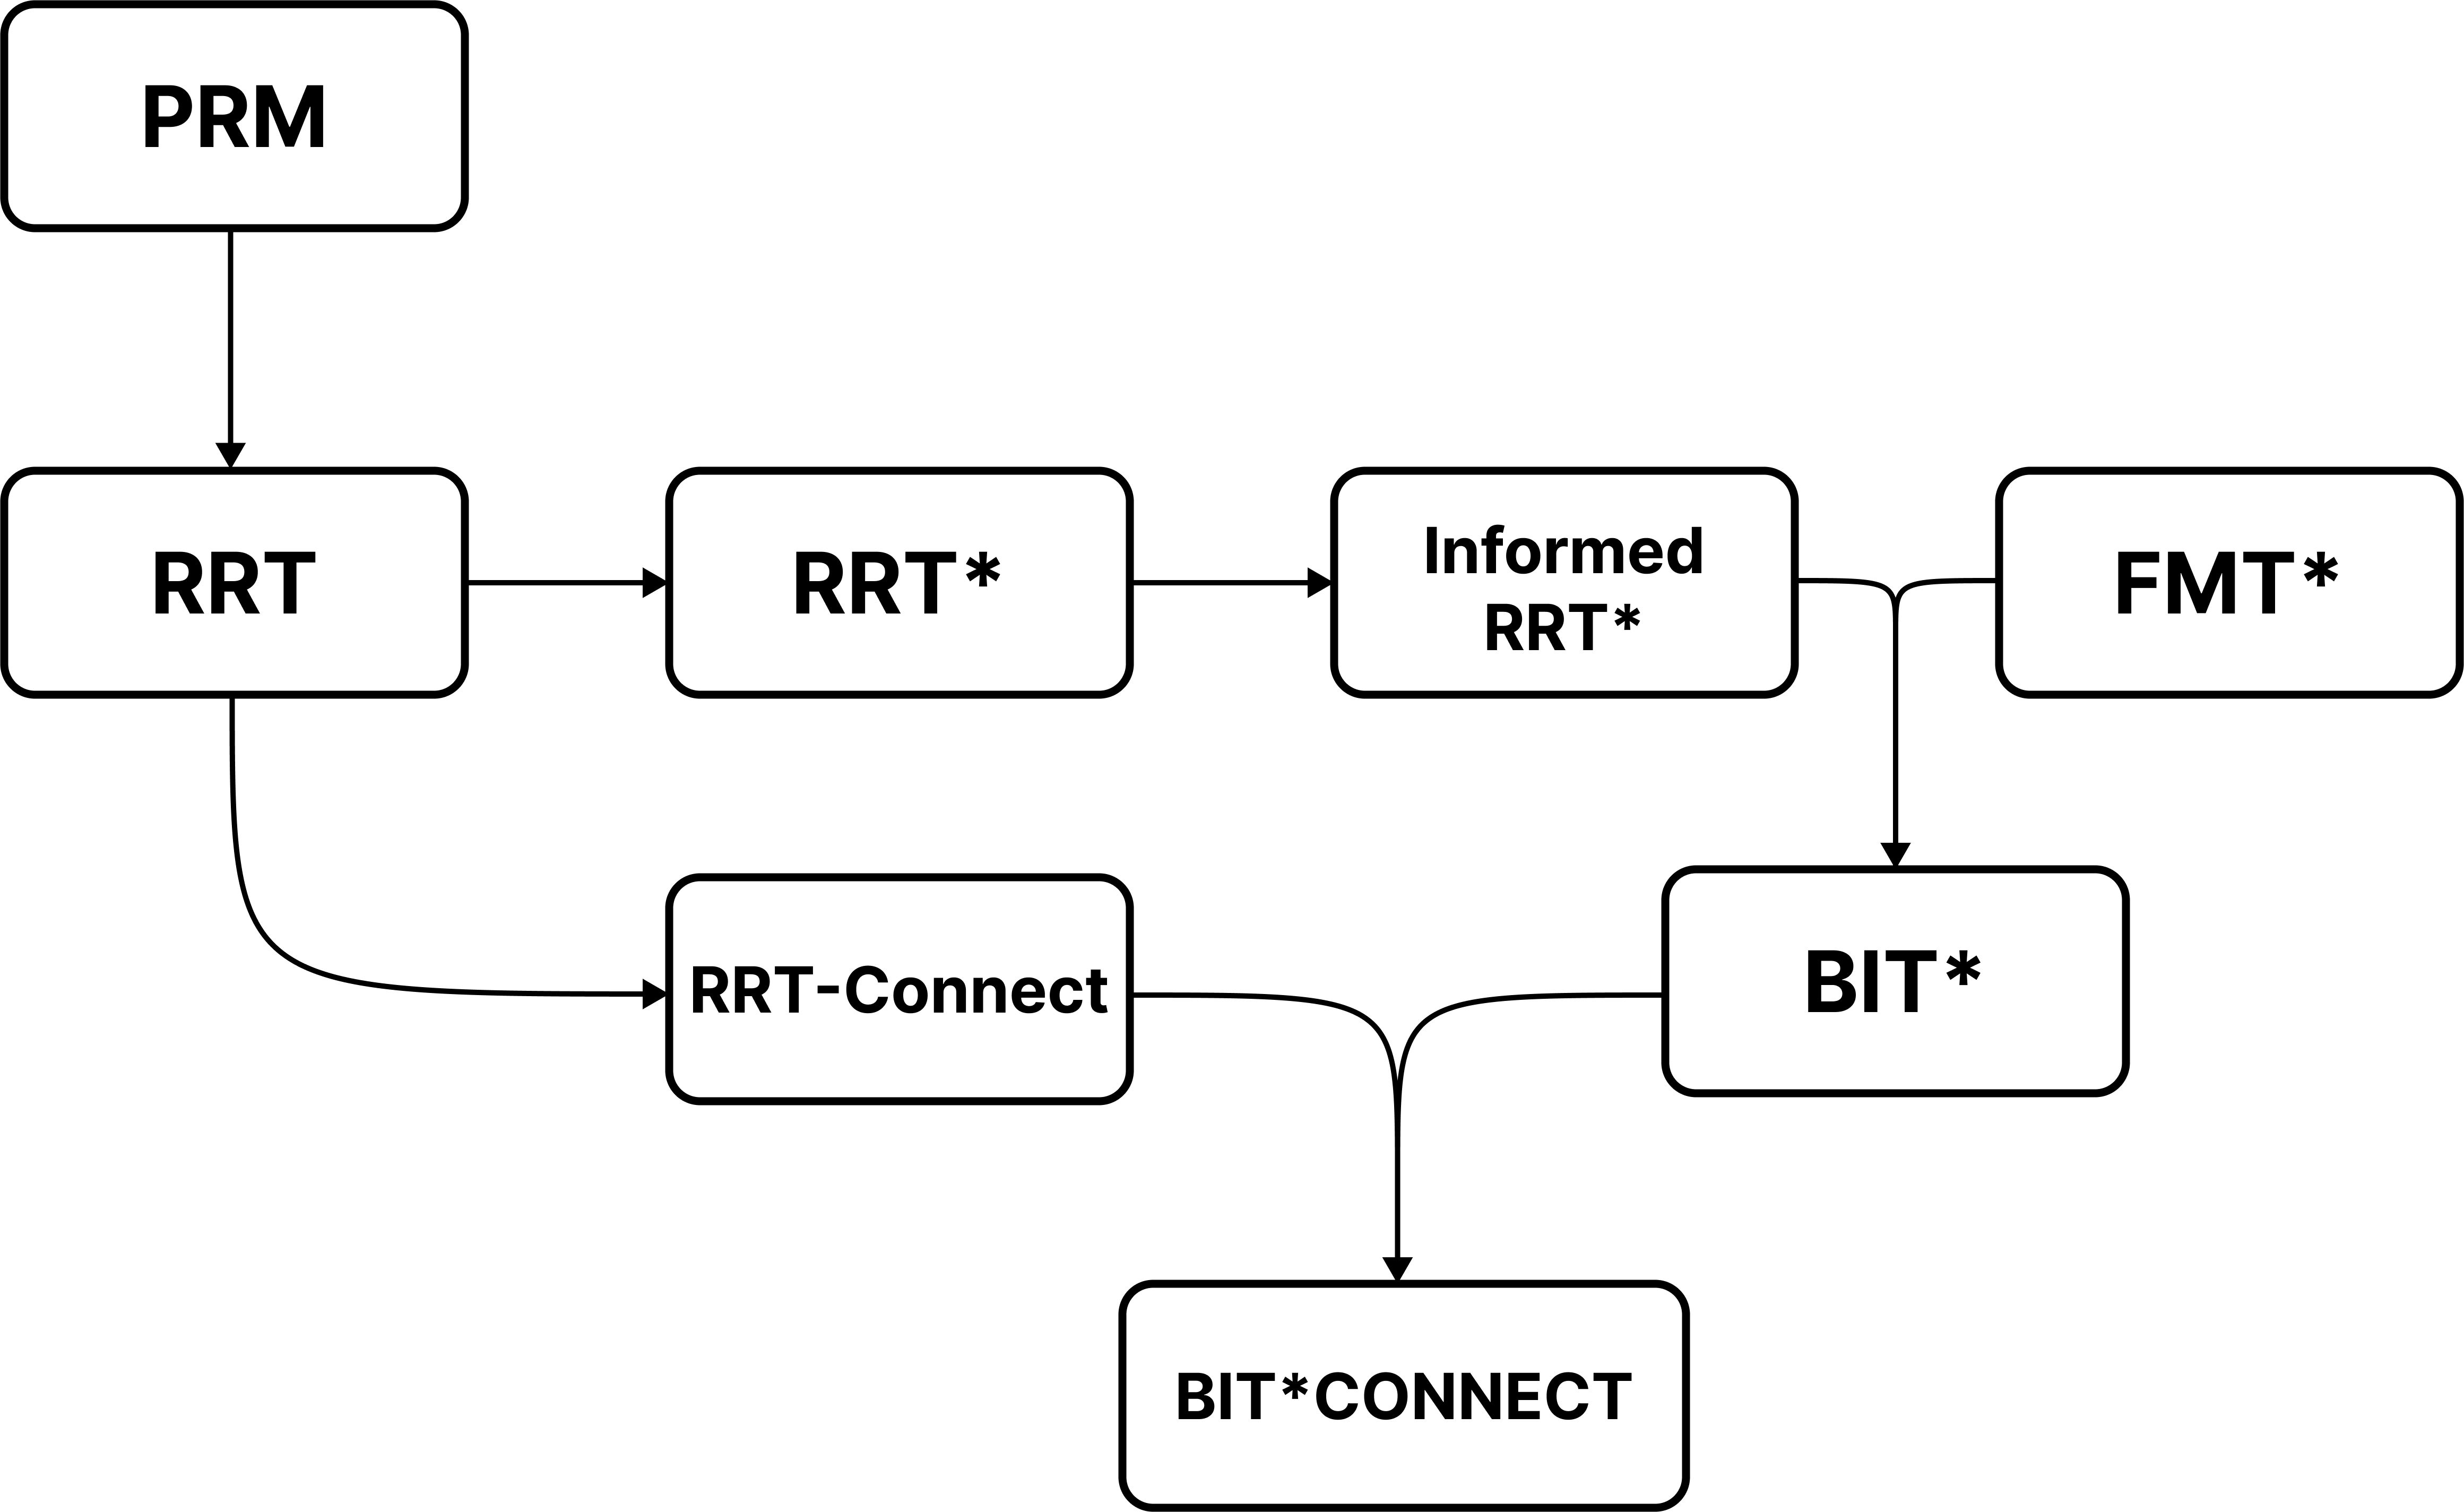
\includegraphics[height=15cm,width = 15cm]{Flow.png}




\chapter{Progress}

\section{WEEK 1}
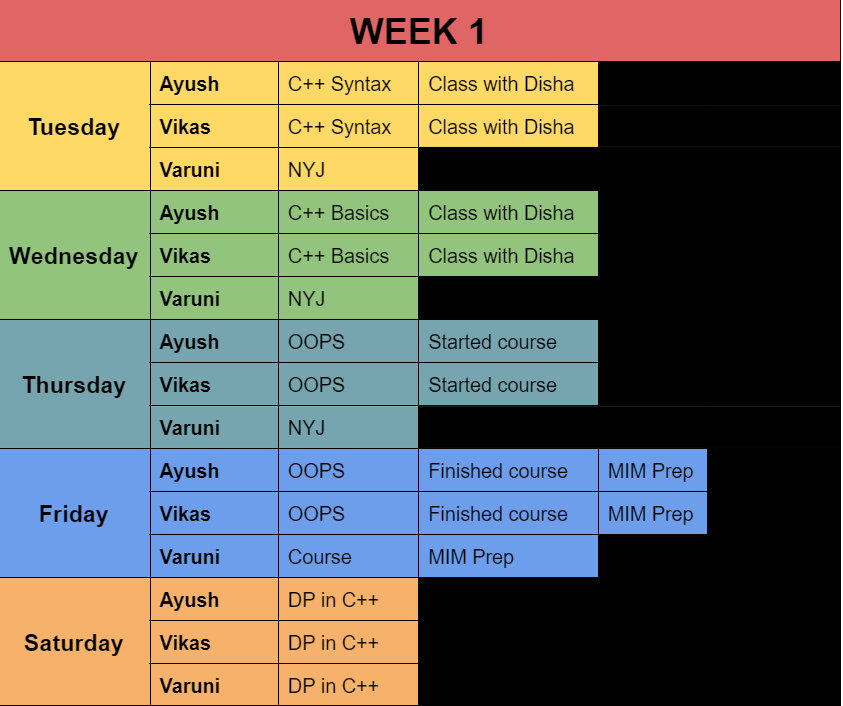
\includegraphics[height=11cm,width = 15cm]{week1.png}

\section{WEEK 2}
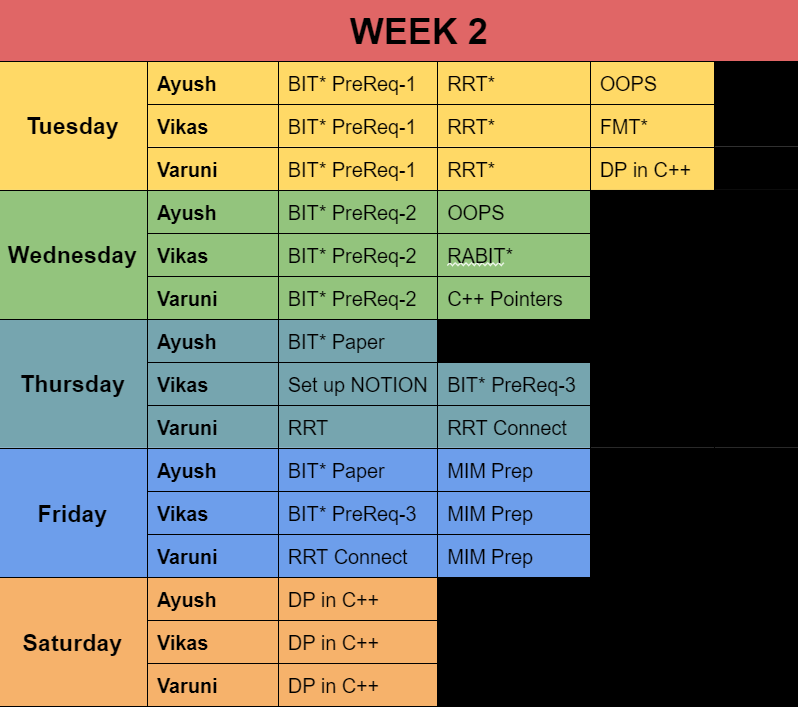
\includegraphics[height=17cm,width = 15cm]{week2.png}
\section{WEEK 3}
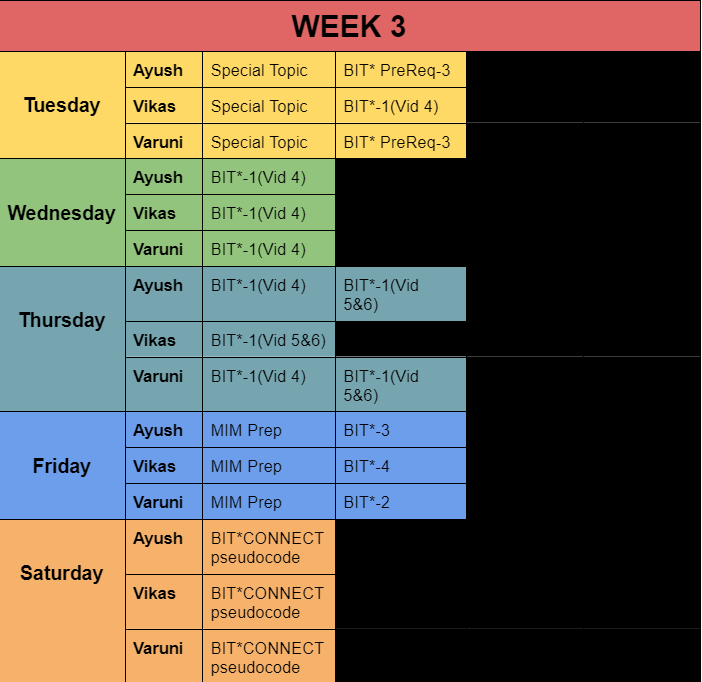
\includegraphics[height=17cm,width = 15cm]{week3.png}
\section{WEEK 4}
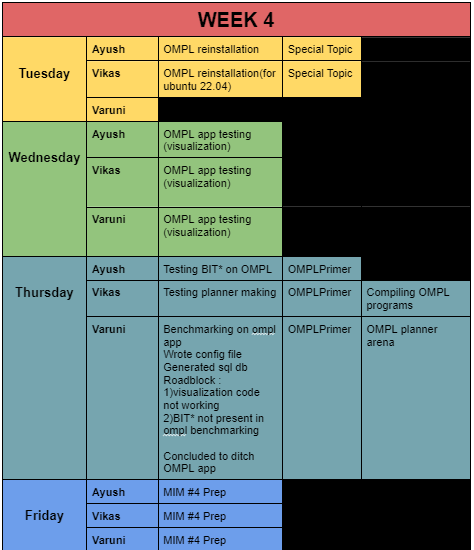
\includegraphics[height=17cm,width = 15cm]{week4.png}

% \chapter{Main Body}
% This is the heart of your report. It describes your project. It can be more than one chapter/section. For example : 'System model', 'methodology', 'solution method', 'approach'. Include diagrams, flow charts, algorithms etc. if relevant. Make sure you refer to all figures and tables that you include in the text. Like this: In Figure \ref{solvay}, the IQ level is over 9000! (Read in Vegeta voice.)
% %template for figure

% \begin{figure}[ht]
%   \includegraphics[width =\columnwidth]{solvay.jpg}
%   \caption{Some inspiration}
%   \label{solvay}
% \end{figure}

% \section{Hardware and Software Requirements}
% We are using the Open Motion Planing Library as it contains most motion planners and it has a testbench to benchmark our algorithms


% \section{Artifacts}
% What are the Inputs that your system requires? In an Ideal Scenario, what are the outputs? How do certain inputs impact the output, if there exists such a mapping? Do add in a workflow diagram of the system to ease explanation and improve understanding. 

% \chapter{Results and Discussion}
% Include tables (see Table \ref{XYComparison} for a template), figures and plots to represent your results if possible. What were the key outcomes? Do they match with expected results? Why/why not? Discuss and explain results where possible. Talk about challenges faced and the limitations of the present implementation if any. 


%template for table
 
 

\chapter{Conclusions and Future Work}
%A short paragraph about the conclusions you have drawn. Feel free to change the formatting and sizes of your figures/tables. In conclusion, your report should a) give the reader an idea of what you did b) allow them to understand and replicate your results.
The conclusion we draw from this report is that intuitively, BIT*Connect should be able to combine the "Elliptical Guiding" function of BIT* and the "Connect" function of RRT-Connect to create a Bidirectional BIT*Connect.
\vspace{5pt}

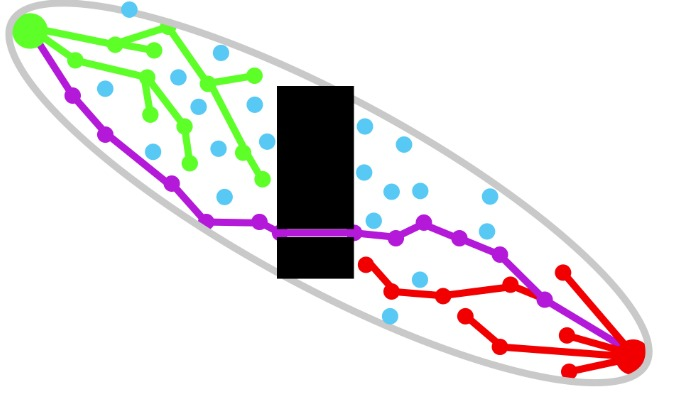
\includegraphics[height=5.75cm,width = 10.75cm]{bitconnect.png}
%Please make sure you keep a log of all the resources you have used. This includes websites, tutorials, videos, papers or even blogs can be cited.

\bibliographystyle{ieeetr} 
\bibliography{bibmil.bib}
\appendix 

%\label{app_1}
 
\chapter{Appendex}
open motion planning library \href{https://ompl.kavrakilab.org/}{https://ompl.kavrakilab.org/}
 \vspace{2pt}
 
     Benchmarking - pathbench \href{https://github.com/perfectly-balanced/PathBench}{https://github.com/perfectly-balanced/PathBench}
 
 


\end{document}
